\chapter{Sprint 4: Data visualization \& projects management}
In this chapter, we focus on Sprint 4, which is dedicated to enhancing data visualization and project management within our application. This sprint aims to develop and implement functionalities for visualizing data and managing projects effectively.

Advanced data visualization techniques will enable users to gain insights from complex datasets, while robust project management tools, such as a Scrumboard, will facilitate the planning, execution, and monitoring of various projects. We will explore the processes involved in these functionalities to ensure they are intuitive and efficient. 

By leveraging these advanced visualization techniques and project management features, we aim to enhance user experience and optimize project workflows.
\pagebreak

\section{Analysis of Sprint 4 Requirements}
In this section, we will analyze the requirements for Sprint 4, which focuses on container management. This sprint involves developing and implementing functionalities related to container images, including fetching images, instantiating containers, and managing container clusters. 

\subsection{Use cases diagram of Sprint 4}

The following figure (\hyperref[fig:sprint_use_cases4]{Figure \ref{fig:sprint_use_cases4}})  represents the uses cases of our sprint.
\begin{figure}[h]
  \center
%\hspace*{-0.9in}
  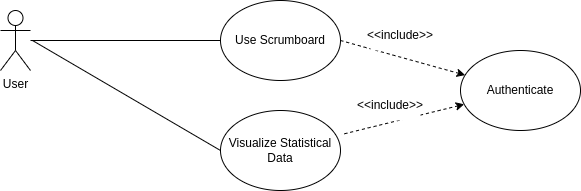
\includegraphics[width=10cm]{./chapters/sprint4/sprint_use_cases.png}
  \caption{Sprint use cases diagram}
  \label{fig:sprint_use_cases4}
\end{figure}

\subsection{Interfaces}
In this section, we will provide some screenshots of our application interfaces. These screenshots will illustrate the various functionalities and processes related to user management as part of Sprint 1, as well as managing vault secrets. 

The following figure (\hyperref[fig:login]{Figure \ref{fig:login}})  depicts the login page of our application.
\begin{figure}[h]
  \center
%\hspace*{-0.9in}
  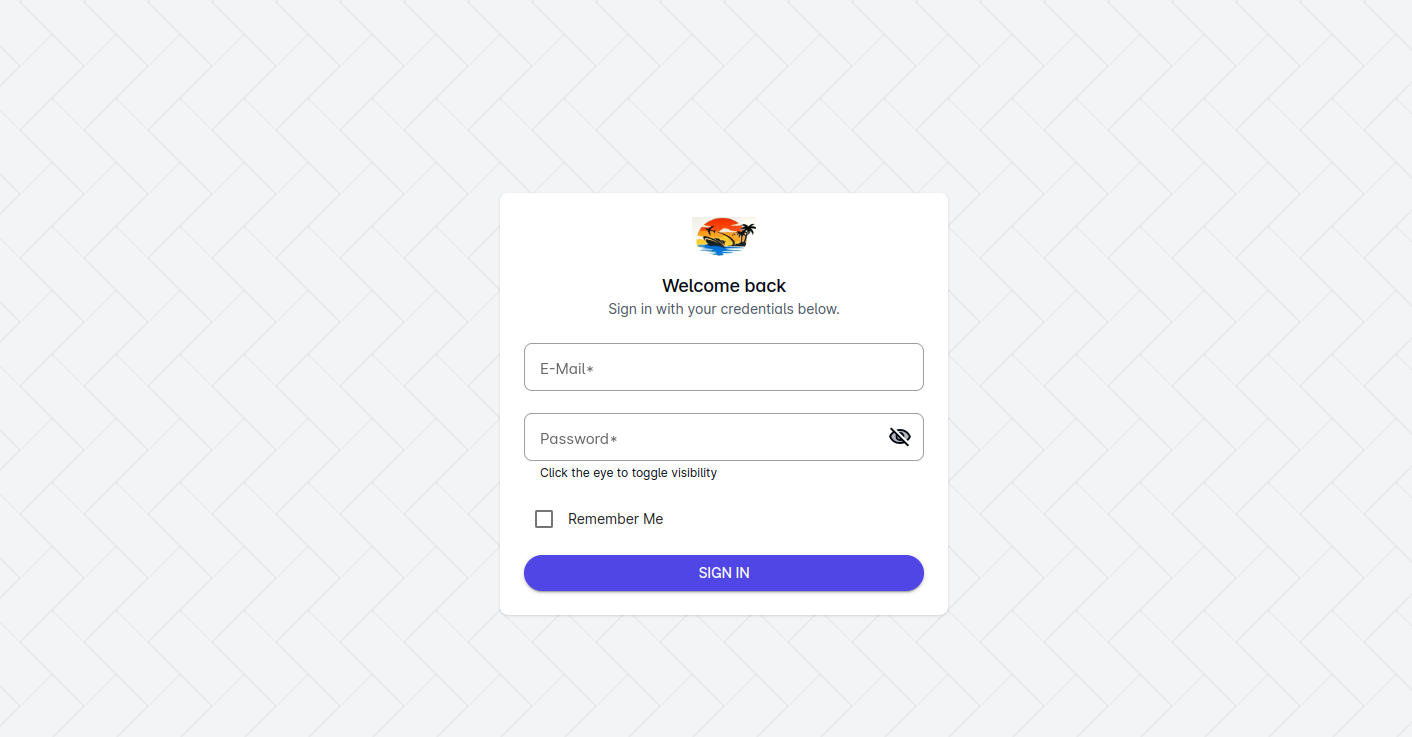
\includegraphics[width=10cm]{./chapters/sprint1/login.png}
  \caption{Ilef login pagelef login page}
  \label{fig:login}
\end{figure}

\subsection{Sequence diagram of "Visualize Statistical Data" use case}

The following figure (\hyperref[fig:sequence-data]{Figure \ref{fig:sequence-data}})  represents the ``Visualize Statistical Data'' sequence diagram.
\begin{figure}[h]
  \center
%\hspace*{-0.9in}
  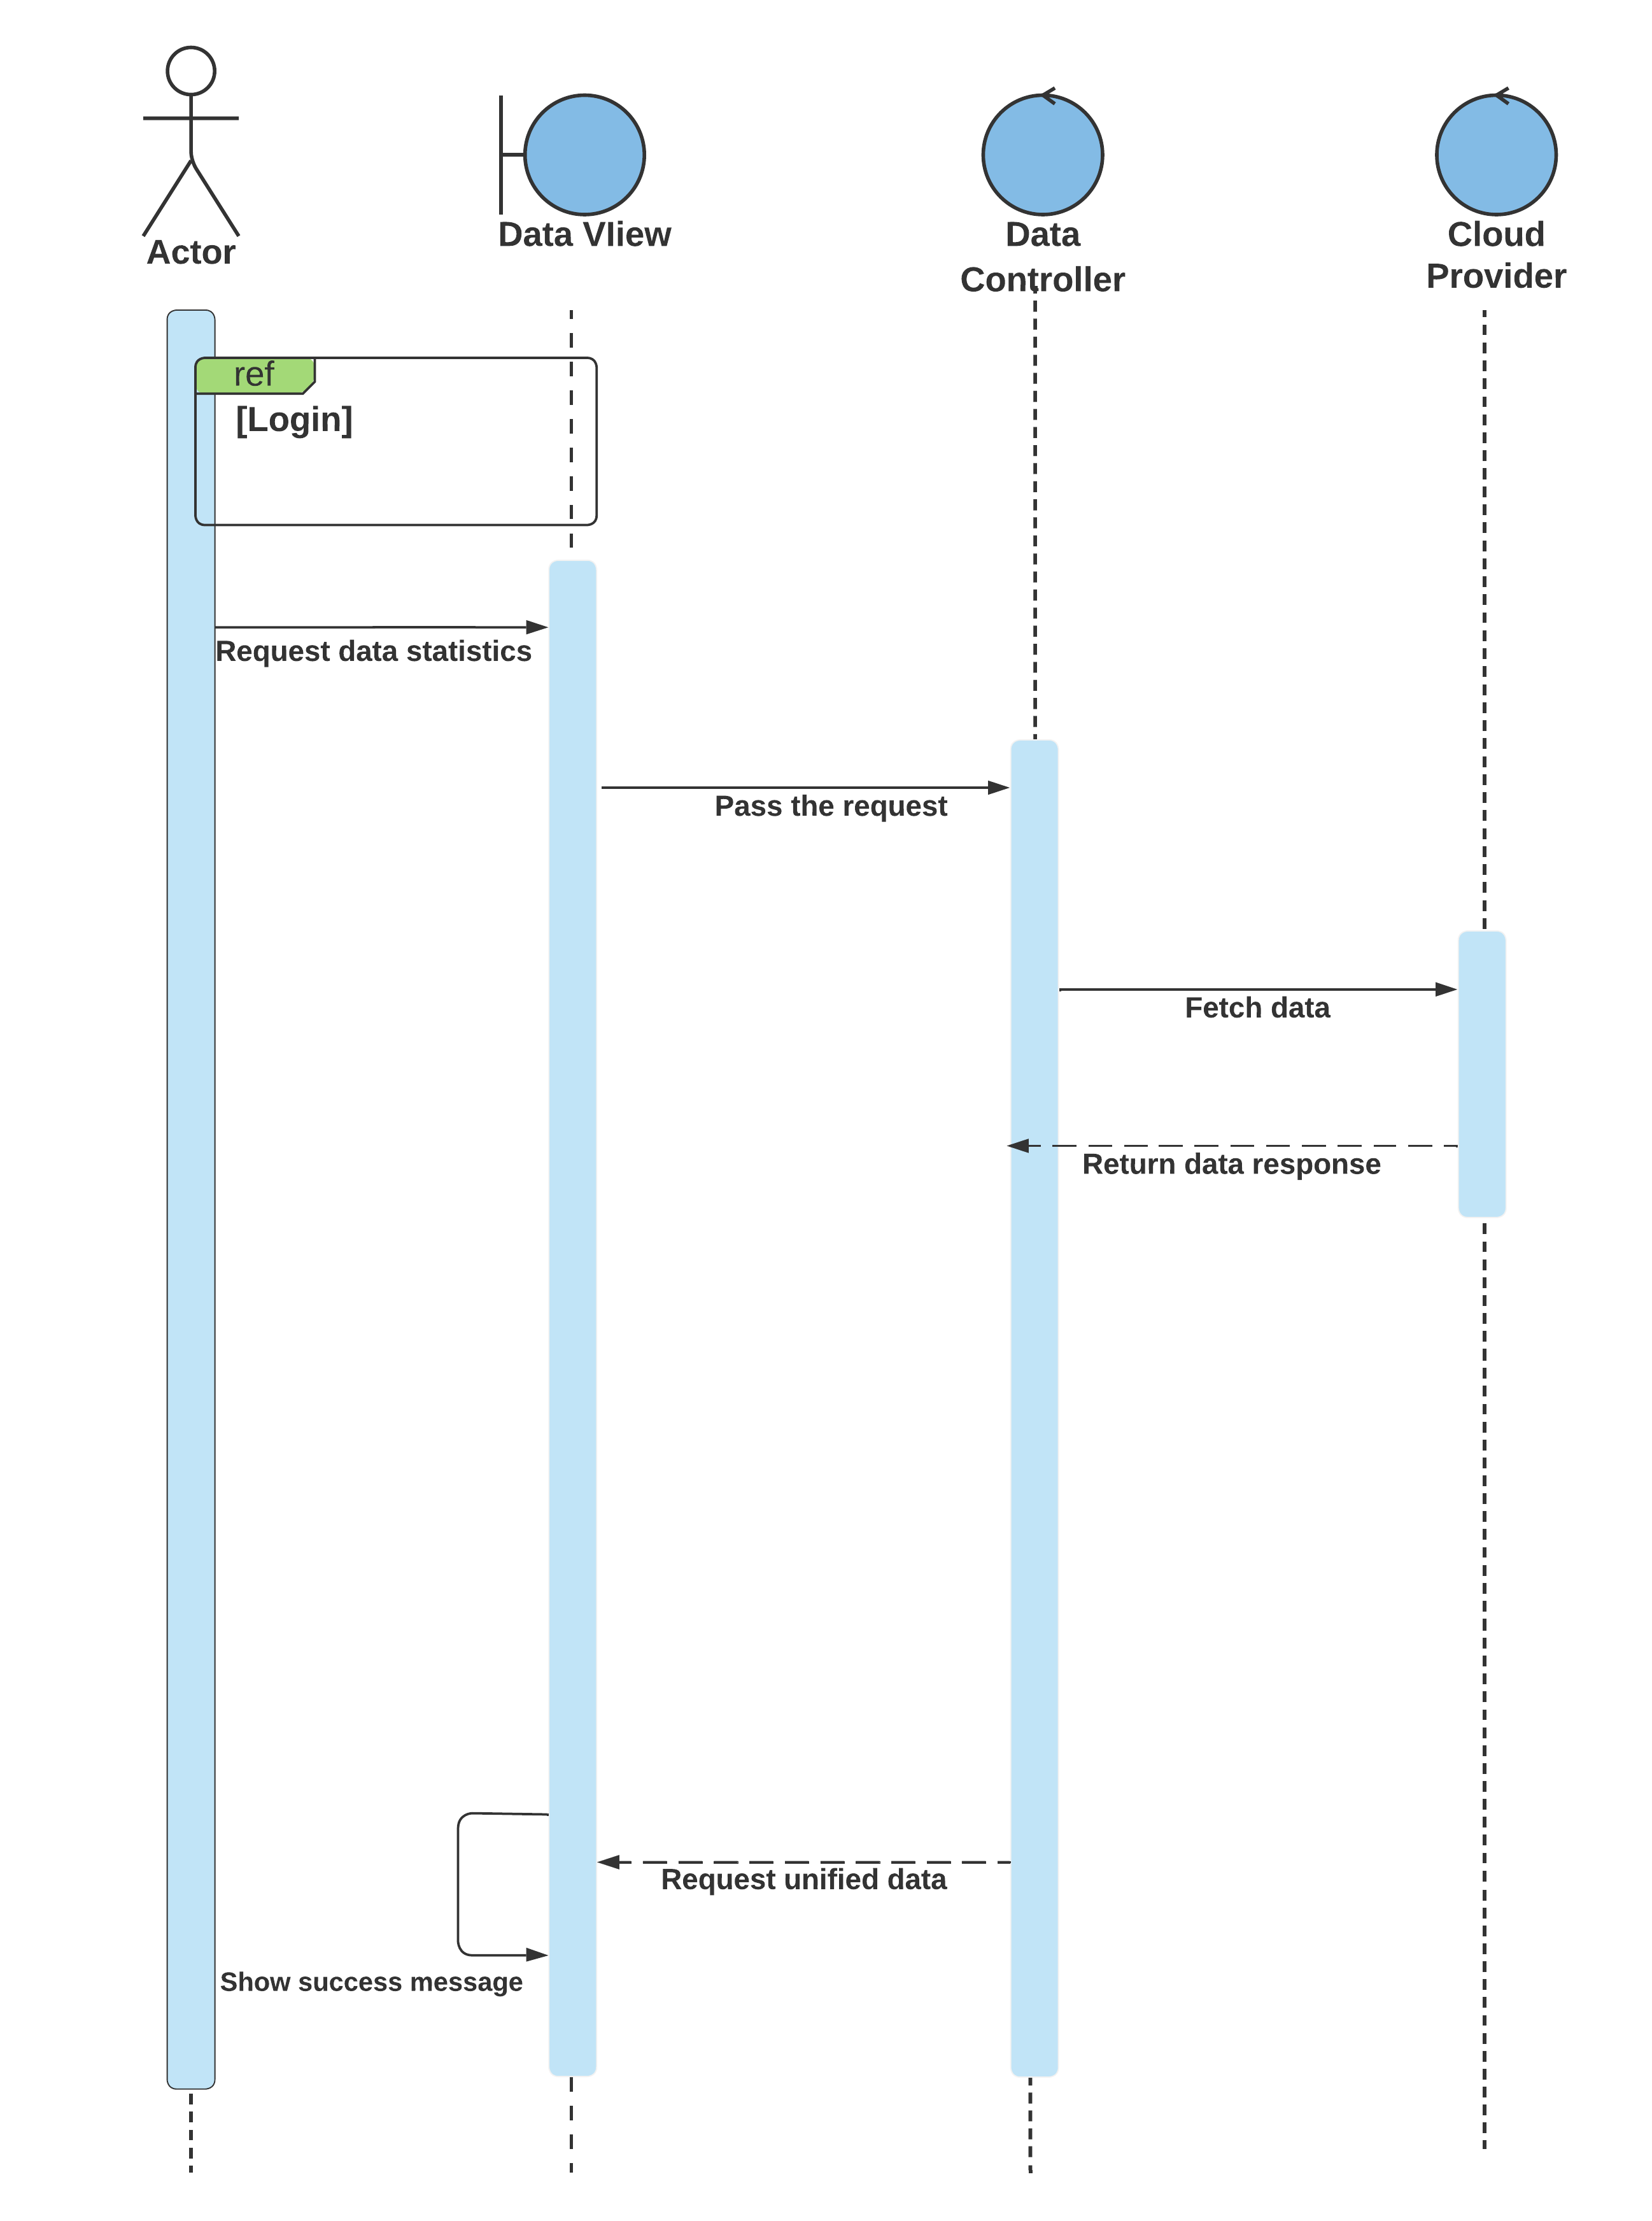
\includegraphics[width=14cm]{./chapters/sprint4/sequence-data.png}
  \caption{Sequence diagram: Instantiate Container}
  \label{fig:sequence-data}
\end{figure}

\subsection{Interfaces}
In this section, we will provide screenshots and detailed explanations of the interfaces related to data visualization and project management as part of Sprint 4. These interfaces cover the functionalities for creating and viewing data visualizations, managing projects, and utilizing Scrumboards.


The following figure (\hyperref[fig:data-visualization]{Figure \ref{fig:data-visualization}}) represents the data visualization page of our application, which serves as our landing page.


\begin{figure}[h]
  \center
%\hspace*{-0.9in}
  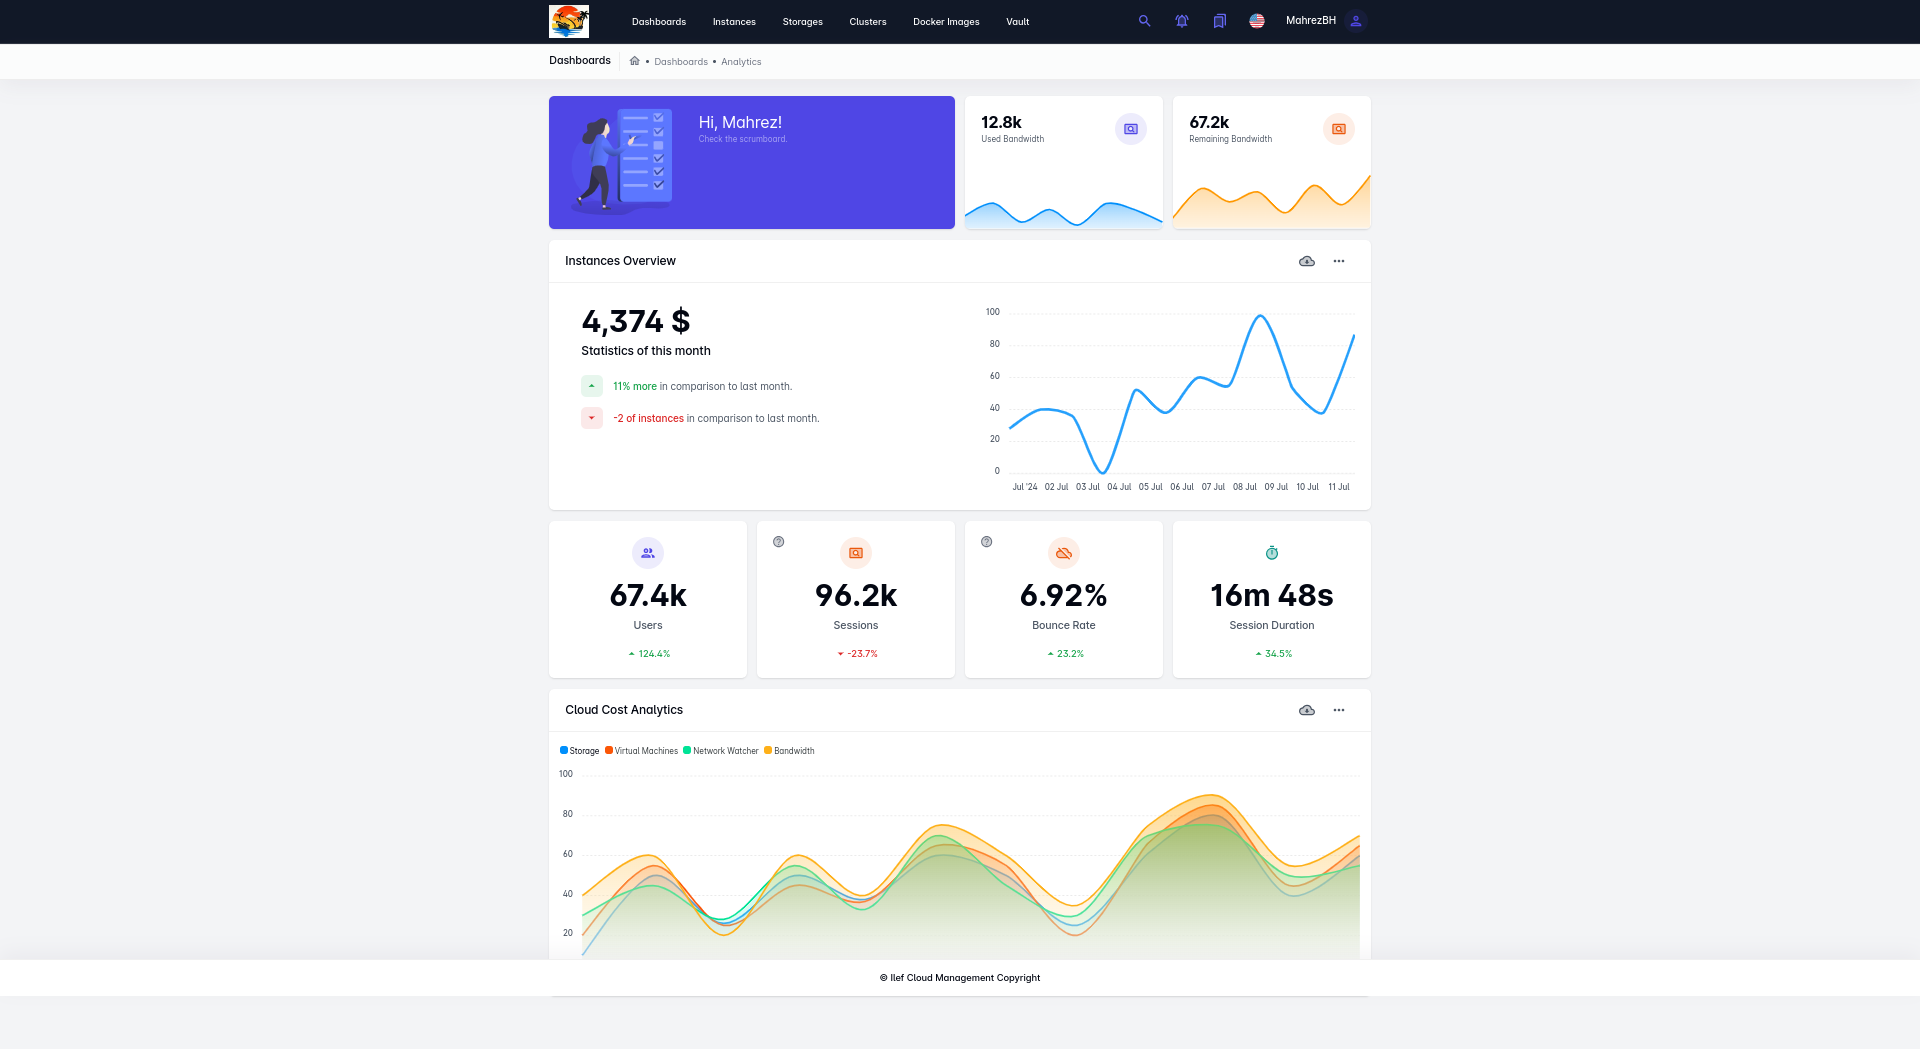
\includegraphics[width=13cm]{./chapters/sprint4/landing page.png}
  \caption{Ilef data visualization page}
  \label{fig:data-visualization}
\end{figure}

The following figure (\hyperref[fig:scrumboard]{Figure \ref{fig:scrumboard}})  represents the Scrumboard of our application.
\begin{figure}[h]
  \center
%\hspace*{-0.9in}
  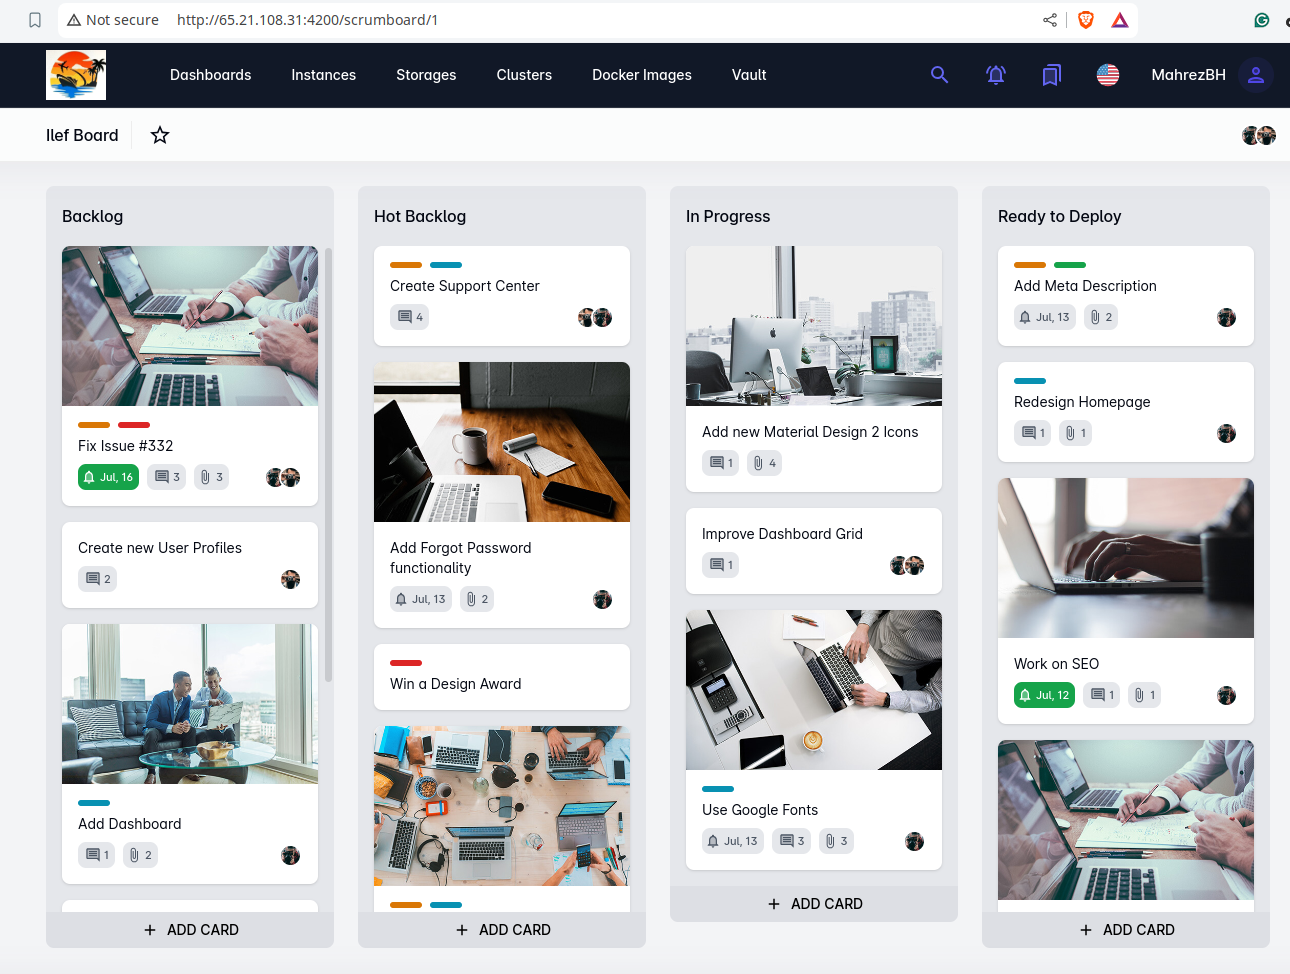
\includegraphics[width=13cm]{./chapters/sprint4/scrumboard.png}
  \caption{Ilef Scrumboard page}
  \label{fig:scrumboard}
\end{figure}

\section*{Conclusion}
In this chapter, we focused on Sprint 4, which concentrated on data visualization and project management. We developed and implemented functionalities that enable users to create and view various data visualizations, efficiently manage projects, and utilize Scrumboards for agile project management.

We provided detailed interfaces for data visualization, project management, and Scrumboard functionality, demonstrating how users can interact with these tools to gain insights, plan, execute, and monitor their projects. These features enhance the user experience and improve workflow efficiency, ensuring that our application effectively meets user needs.

By completing Sprint 4, we have significantly enhanced our application's capabilities in data visualization and project management, establishing a strong foundation for future development and optimization
